%=====================================================================
\section{Hypotheses}\label{sec:hypotheses}
Table~\ref{tab:hyp} states three primary hypotheses, two supporting ones and one registered test, each with the outcome that would refute it. The first draft of this paper listed seven hypotheses for six funds; the list is cut so that each claim rests on a test the data can bear. All except R1 were written after the price path of September and October 2026 was public (Appendix~\ref{app:protocol}).

\begin{table*}[!t]
\centering\footnotesize
\caption{Hypotheses, tests and refutation conditions}\label{tab:hyp}
\begin{tabularx}{\textwidth}{L{1.55cm}L{3.9cm}YL{3.9cm}}
\toprule
 & Statement & Test & Refuted if\\
\midrule
\multicolumn{4}{l}{\emph{Primary}}\\
P1 Rule effect & From 7 September 2026 the premium of rationed funds rises against its own history and against domestic equity ETFs, and the break falls on the rule date & Rank of each fund's return on 7 September, a US holiday, within its daily returns since 2023; break-date search by fund; event-study statistic recomputed for every date since January 2023; intervals for few treated groups with domestic ETFs as controls & The break lies more than two sessions from 7 September in half or more of the US-linked rationed funds; or domestic ETFs break by a similar amount; or the true date is outside the top 1\% of placebo dates\\
P2 Hidden premium & Before the change the premium was censored at the day's ceiling; after it, the realised premium exceeds a forecast of the latent premium & Censored autoregression to 4 September with the official ceiling; forecast from 7 September; induced share over sessions 16 to 40 & Two-sided. Realised premium inside the 90\% forecast band: the rule revealed demand. Above it: the rule induced demand\\
P3 Supply and float & The premium falls after a creation, and across funds it is lower where net float is larger & Event study over sessions $-5$ to $+10$ around each dated creation, scaled by the percentage change in units; rank correlation of premium and net float & The mean change after creations is zero or positive; or the rank correlation among US-linked funds is positive\\
\addlinespace
\multicolumn{4}{l}{\emph{Supporting}}\\
S1 Limit-hit dynamics & After an upper-limit day: a positive return next day, more trades and smaller trades; premium changes follow the fund's own lagged return after controlling for turnover & Regression~\eqref{eq:s1} with day-after-limit indicators & No continuation; or a coefficient on the lagged return at or below zero\\
S2 Feeders & Feeder funds shed ETF units when the premium is high & Monthly change in units held by feeders against the lagged premium; descriptive & Feeder holdings rise in high-premium months\\
\addlinespace
\multicolumn{4}{l}{\emph{Registered}}\\
R1 April 2027 & If a NAV anchor is applied on 1 April 2027 the premium collapses before the date in a run, not on the date in a jump & Section~\ref{sec:april} & By branch; Section~\ref{sec:april}\\
\bottomrule
\end{tabularx}
\end{table*}

%=====================================================================
\section{Data and Measurement}\label{sec:data}
\subsection{Funds and comparison groups}
The study covers the six India-listed ETFs that hold foreign equity (Table~\ref{tab:funds}). Two comparison groups are used. Domestic equity ETFs from several fund houses faced the same change of band with creation open, and control for the rule. China-listed quota ETFs on the Nasdaq-100 and S\&P~500 faced the same underlying markets under a different rule, a 10\% limit on the previous close with trading halts, and control for a global rush into US technology shares. Gold and silver ETFs have a different band and are not used as controls. The sample is daily, from January 2021 to June 2027.

\begin{table*}[!t]
\centering\footnotesize
\caption{The six funds}\label{tab:funds}
\begin{tabularx}{\textwidth}{L{2.25cm}L{2.1cm}YR{1.5cm}R{1.45cm}R{1.5cm}R{1.6cm}}
\toprule
Fund (NSE symbol) & Fund house & Index & Listed & Creation unit & Units, million & Value at NAV, Rs crore\\
\midrule
\fund{MONQ50} & Motilal Oswal & Nasdaq Q-50 & Dec 2021 & 600,000 & 14.68 & 168\\
\fund{MON100} & Motilal Oswal & Nasdaq-100 & Mar 2011 & 250,000 & 504.13 & 12,911\\
\fund{MASPTOP50} & Mirae Asset & S\&P 500 Top 50 & Sep 2021 & n.e. & 168.62 & 1,082\\
\fund{MAFANG} & Mirae Asset & NYSE FANG+ & May 2021 & n.e. & 247.30 & 3,945\\
\fund{MAHKTECH} & Mirae Asset & Hang Seng TECH & Dec 2021 & 800,000 & 193.71 & 315\\
\fund{HNGSNGBEES} & Nippon India & Hang Seng & Mar 2010 & 25,000 & 23.59 & 1,030\\
\bottomrule
\end{tabularx}
\tabnote{Units outstanding and NAV are for 9 November 2026 \citep{nse2026files,amfi2026nav}. Listing dates are from NSE's list of ETFs. Creation-unit sizes are from scheme documents and project records; changes in units outstanding are exact multiples of them (Table~\ref{tab:units}). n.e.: not yet established.}
\end{table*}

\subsection{Sources}
Daily prices, volume, number of trades and delivered quantity come from NSE's full bhavcopy, available from January 2021, and the equivalent BSE file. NSE's daily security master carries two fields on which much of the design rests: the official price band for each ETF's next session and its units outstanding \citep{nse2026files}. The first gives the exact ceiling on each day. The second moves in multiples of the creation unit and so dates every creation and redemption; it is available from July 2024, and monthly assets divided by NAV fill the earlier period. Daily NAVs are from the Association of Mutual Funds in India \citep{amfi2026nav}. Index futures and exchange rates at the Indian close come from a terminal, intraday prices and iNAV from a recorder that the project runs, feeder holdings from fund houses' monthly portfolios, search interest from Google Trends pulled in fixed overlapping windows, and dated events from regulators' and exchanges' publications. As of 12 November 2026 each public source has been checked against live files and its format recorded; the collectors and the clean panel are being built. Code and derived variables will be released. Licensed data will not be redistributed.

\subsection{Premium measures}
The premium quoted in the press is
\begin{equation}\label{eq:raw}
\pi^{\mathrm{q}}_{i,t}=\frac{P_{i,t}}{\NAV_{i,t}}-1,
\end{equation}
with both terms dated $t$. For a US-linked fund the denominator is fixed after the numerator (Figure~\ref{fig:timeline}). Let $a(t)$ be the date of the last NAV whose underlying market had closed before the Indian close on $t$: normally $t-1$ for a US-linked fund and $t$ for a Hong Kong fund. Fair value at the Indian close is
\begin{equation}\label{eq:fv}
\FV_{i,t}=\NAV_{i,a(t)}\times\left(\frac{F^{\,\mathrm{IN}}_{t}}{F^{\,\mathrm{cl}}_{a(t)}}\right)^{\beta_i}\times\frac{S^{\,\mathrm{IN}}_{t}}{S^{\,\mathrm{cl}}_{a(t)}},
\end{equation}
where $F$ is the front index future and $S$ the rupee exchange rate, each observed at 15:30 Indian time on $t$ (superscript IN) and at the underlying market's close on $a(t)$ (superscript cl). Three of the indices are not those the liquid futures track, so results are reported with $\beta_i=1$ and with $\beta_i$ estimated as the slope of the fund's NAV return, net of currency, on the future's return over the 250 NAV dates before the change. The main dependent variable is the log premium
\begin{equation}\label{eq:pi}
\pi_{i,t}=\ln\!\left(\frac{P_{i,t}}{\FV_{i,t}}\right).
\end{equation}
Logs keep a 235\% observation from dominating. The premium over the last known NAV, $P_{i,t}/\NAV_{i,a(t)}-1$, uses no futures and is reported alongside.

\subsection{The ceiling and limit days}
Let $U_{i,t}$ be the official upper limit for session $t$, read from the security master of the previous session. The ceiling on the fair-value premium is
\begin{equation}\label{eq:cap}
c_{i,t}=\ln\!\left(\frac{U_{i,t}}{\FV_{i,t}}\right),
\end{equation}
the empirical counterpart of~\eqref{eq:fence}. The first draft treated the ceiling as a fixed ratio of 1.2 to the NAV of $t-2$. That ratio is fixed, but the premium over fair value that it allows is not, and it is the latter that demand acts on. NSE's closing price is an average over the last half hour, so a close at the limit cannot be read from the close alone. Three indicators are kept for each side: the day's high reached the initial limit; it reached the maximum limit; the last trade was at the limit. Minute bars and order-book snapshots, where available, separate a limit that was touched from one at which the book was empty on the other side.

\subsection{Rationing, float and turnover}
A creation or redemption is a change in units outstanding, measured in creation units. A fund-day is \emph{rationed} when the premium exceeds 2\% and no unit has been created in the previous 20 sessions; the threshold is varied from 1\% to 5\%. This replaces a fixed label by fund: Section~\ref{sec:evidence} shows that creation in some funds continued long after the dates on which the press reports it stopped. Net float is units outstanding less units held by feeder funds, valued at the last known NAV. Turnover is units traded on both exchanges over units outstanding; a rupee turnover would mix in the premium. Appendix~\ref{app:variables} lists every variable.

%=====================================================================
\section{Empirical Design}\label{sec:design}
\subsection{The rule effect (P1)}
The cleanest observation is the first day. On 7 September 2026 US markets were closed for Labor Day, so the value of the US-linked funds could not move except through the rupee, and the band changed. Any change in price that day is a rule effect with value held fixed. Following the logic of single-event inference \citep{gelbach2013valid}, each fund's return on 7 September is ranked within the empirical distribution of its own daily returns since January 2023, and the same is done for domestic ETFs.

Three further tests rely on timing. A search for an unknown break date in each fund's premium \citep{bai1998estimating} should select 7 September in the rationed funds and no nearby date in the controls. An event study,
\begin{equation}\label{eq:event}
\begin{split}\pi_{i,t}&=\alpha_i+\lambda_t\\&\quad+\sum_{k\neq -1}\beta_k D^{k}_{i,t}+\varepsilon_{i,t},\end{split}
\end{equation}
where $D^{k}_{i,t}$ equals one for a rationed fund in week $k$ relative to the rule date, gives a path of coefficients; its test statistic is recomputed for every possible date since January 2023 to place the true date in a placebo distribution. And the difference between rationed funds and domestic ETFs is given intervals built for a small number of treated groups \citep{conley2011inference,ferman2019inference}.

\subsection{The hidden premium and the induced share (P2)}
For each fund the latent premium is modelled on the sample to 4 September 2026 as
\begin{align}
\begin{split}\pi^{*}_{i,t}&=\mu_i(1-\rho_i)+\rho_i\,\pi^{*}_{i,t-1}\\&\quad+x_t'\gamma_i+\sigma_i\varepsilon_{i,t},\end{split}\label{eq:latent}\\
\pi_{i,t}&=\min\big(\pi^{*}_{i,t},\,c_{i,t}\big),\label{eq:obs}
\end{align}
with $\varepsilon_{i,t}\sim N(0,1)$, $c_{i,t}$ from~\eqref{eq:cap} and $x_t$ the five-day return of the underlying index, the return on the Nifty, the change in the rupee and search interest. A day is treated as capped when the high reaches the official limit. The model is a Tobit \citep{tobin1958estimation} with two features that the application requires. The censoring point is observed and differs every day. And the lag in~\eqref{eq:latent} is the latent premium, not the observed one: what buyers would have paid yesterday, had they been allowed to, carries over to today. Over a run of capped days the lagged state is unobserved, so the likelihood integrates it out \citep{lee1999estimation}. Because the state is one-dimensional the integral is computed directly. If $f_{t-1}$ is the density of $\pi^{*}_{t-1}$ given the data to $t-1$, then on a capped day
\begin{equation}\label{eq:filter}
\begin{split}f_{t}(u)\;\propto\;&\mathbf{1}\{u\ge c_{t}\}\\&\times\int\phi\!\left(\frac{u-\mu(1-\rho)-\rho v-x_t'\gamma}{\sigma}\right)f_{t-1}(v)\,dv ,\end{split}
\end{equation}
and the normalising constant is that day's contribution to the likelihood; on an uncapped day the state is observed and the density collapses to a point. The recursion is run on a grid. Identification comes from stretches in which the premium was free: press data show the Nasdaq 100 ETF at a 22\% premium at the end of December 2024 and at zero in May 2025 \citep{vr2025premium}, so the pre-period contains both regimes.

The filtered density on 4 September, $f_{T_0}$, is the estimate of the \emph{hidden premium} on the last day of the fence. Simulating~\eqref{eq:latent} forward from it gives the forecast distribution of the latent premium in each later session. Let $\widehat{\Pi}^{\,*}_{i}$ be the forecast mean of the premium $e^{\pi^{*}}-1$ averaged over sessions 16 to 40 after the change, and $\overline{\Pi}_{i}$ the realised average over the same sessions. The \emph{induced share} is
\begin{equation}\label{eq:iota}
\iota_i=1-\frac{\widehat{\Pi}^{\,*}_{i}}{\overline{\Pi}_{i}}.
\end{equation}
The first 15 sessions are left out because the price needs time to reach a high latent premium at 20\% a day and because they contain the run-up and crash of one fund; session 40 is 4 November 2026. The window was fixed before any series was computed. The test is two-sided. If the realised average lies inside the 90\% forecast band, the rule revealed demand that the fence had hidden. If it lies above, the rule induced demand. Section~\ref{sec:mc} examines the size and power of this test.

Two variants bound the result. A model in which the lag in~\eqref{eq:latent} is the observed premium lets nothing accumulate behind the fence and gives a lower bound on the hidden premium. And the covariates $x_t$ are entered at their realised post-change values, so that a rise in the underlying index or in search interest is not counted as induced; a version without search interest attributes attention drawn by the rule to the rule.

\subsection{Does the estimator work? A Monte Carlo check}\label{sec:mc}
Before it is taken to data the estimator is tested on simulated data in which the truth is known. Each replication draws a latent premium from~\eqref{eq:latent} without covariates, with $\rho=0.985$ and $\sigma=0.02$, over 400 pre-change sessions and 40 later ones. The ceiling is $\ln 1.2$ less the two-day change in value, where daily changes in value have a standard deviation of 1.2\%. The observed premium is the lower of the two. Three values of the long-run mean $\mu$ give designs in which about \mcShareA\%, \mcShareB\% and \mcShareC\% of days are capped, which spans what press data suggest for the six funds. As in the data, only replications in which the last pre-change day is capped are kept. Three estimators are compared: an autoregression on the observed premium that ignores censoring; a censored autoregression on the premium over the band's base, $\ln(P_t/\NAV_{t-2})$, whose ceiling is fixed at $\ln 1.2$, as in the first draft; and the censored autoregression of~\eqref{eq:latent}--\eqref{eq:filter} on the fair-value premium with the moving ceiling. Appendix~\ref{app:mc} gives details.

\begin{table*}[!t]
\centering\footnotesize\setlength{\tabcolsep}{4.2pt}
\caption{Monte Carlo: recovering a known hidden premium and testing for induced demand}\label{tab:mc}
\begin{tabular}{lrrrrrrrrr}
\toprule
 & \multicolumn{3}{c}{35\% of days capped} & \multicolumn{3}{c}{60\% of days capped} & \multicolumn{3}{c}{80\% of days capped}\\
\cmidrule(lr){2-4}\cmidrule(lr){5-7}\cmidrule(lr){8-10}
 & Ignored & Fixed & Moving & Ignored & Fixed & Moving & Ignored & Fixed & Moving\\
\midrule
\multicolumn{10}{l}{\emph{A. Hidden premium on the last capped day, percentage points}}\\
True value, mean & \multicolumn{3}{c}{29.4} & \multicolumn{3}{c}{31.9} & \multicolumn{3}{c}{37.6}\\
Mean error & $-$9.8 & 2.7 & 1.3 & $-$12.2 & 3.0 & 1.3 & $-$17.8 & 1.6 & $-$0.7\\
Root mean squared error & 12.7 & 9.2 & 7.6 & 15.3 & 11.8 & 11.1 & 22.2 & 13.7 & 13.9\\
Estimated $\rho$ (true 0.985) & 0.954 & 0.967 & 0.979 & 0.874 & 0.959 & 0.972 & 0.758 & 0.959 & 0.970\\
\addlinespace
\multicolumn{10}{l}{\emph{B. Realised premium above the 90\% forecast band, \% of replications}}\\
No induced demand, plug-in & 30.4 & 7.5 & 6.2 & 69.6 & 12.5 & 12.1 & 88.8 & 15.0 & 18.3\\
No induced demand (nominal 5) & 26.2 & 6.7 & 5.8 & 66.7 & 10.4 & 10.4 & 88.8 & 12.1 & 15.4\\
Induced, 30 log points & 100.0 & 87.9 & 89.6 & 100.0 & 88.3 & 91.7 & 100.0 & 88.3 & 95.0\\
Induced, 60 log points & 100.0 & 98.3 & 99.2 & 100.0 & 98.8 & 99.2 & 100.0 & 98.8 & 98.8\\
\addlinespace
\multicolumn{10}{l}{\emph{C. Realised premium below the band, no induced demand (nominal 5)}}\\
\% of replications & 3.3 & 3.8 & 6.7 & 6.2 & 7.1 & 7.9 & 5.0 & 4.2 & 5.0\\
\addlinespace
\multicolumn{10}{l}{\emph{D. Induced share, median, \%}}\\
No induced demand: true 0 & 28 & $-$11 & $-$18 & 39 & $-$1 & $-$2 & 47 & $-$2 & 3\\
30 log points: true 66/61/57 & 76 & 63 & 61 & 77 & 60 & 61 & 77 & 56 & 59\\
60 log points: true 82/79/76 & 87 & 81 & 80 & 87 & 79 & 79 & 87 & 75 & 77\\
\bottomrule
\end{tabular}
\tabnote{240 replications per design; 400 pre-change sessions; forecast window sessions 16 to 40. `Ignored': autoregression on the observed premium. `Fixed': censored autoregression on the premium over the band's base with ceiling $\ln 1.2$. `Moving': censored autoregression on the fair-value premium with the day's ceiling. Panel A compares the estimated hidden premium on the last pre-change day, which is capped in every replication, with the true latent premium. Panels B and C count replications in which the realised average log premium lies outside the 90\% forecast band; except in the row marked plug-in, the band allows for parameter uncertainty by drawing parameters from their estimated asymptotic distribution. In Panel D the three true values are for the three designs in order. Simulated data; details in Appendix~\ref{app:mc}.}
\end{table*}


Table~\ref{tab:mc} and Figure~\ref{fig:mc} report the results from \mcReps{} replications of each design. Four findings shape the application.

First, ignoring censoring is badly wrong. It understates the hidden premium on the last capped day by \mcBiasNaiveA{} to \mcBiasNaiveC{} percentage points on average, because it takes the ceiling for the premium, and it underestimates persistence. Under pure revelation it then places the realised premium above its forecast band in \mcSizeNaiveMin\% to \mcSizeNaiveMax\% of replications and reports a median induced share of \mcIotaNaiveMin\% to \mcIotaNaiveMax\% when the true share is zero. A researcher who took the pre-change premium at face value would attribute to the rule a premium that the fence had been hiding.

Second, both censored estimators recover the hidden premium with little bias: the mean error is between \mcBiasMovMin{} and \mcBiasMovMax{} points with the moving ceiling and between \mcBiasFixMin{} and \mcBiasFixMax{} with the fixed one. The moving ceiling is more precise when few days are capped (a root mean squared error of \mcRmseMovA{} points against \mcRmseFixA) and no better when most are (\mcRmseMovC{} against \mcRmseFixC). The gain from modelling the ceiling exactly is therefore modest in these designs. The moving ceiling remains the primary specification because it is stated in the premium that demand acts on and is the only one of the two that forecasts the fair-value premium directly; the fixed-ceiling model is reported as a check.

Third, the forecast test has power. When 30 log points of induced demand are added after the change, the realised average lies above the band in \mcPowMovLoMin\% to \mcPowMovLoMax\% of replications, and with 60 log points in \mcPowMovHiMin\%. The estimated induced share is close to its true value in those cases.

Fourth, the test over-rejects when most days are capped, and the application must correct for it. Under pure revelation the realised premium falls above a band that allows for parameter uncertainty in \mcSizeMovMin\% to \mcSizeMovMax\% of replications, against a nominal 5\%, and above a plug-in band in up to \mcPlugMovMax\%. With persistence near one, 400 sessions say little about the long-run mean, and the asymptotic approximation understates that. The application will therefore take its critical values from a parametric bootstrap of the whole procedure under the estimated null, using each fund's actual sequence of ceilings, and will report the simulated size at that fund's capped share beside every test.

\begin{figure*}[!t]
\centering
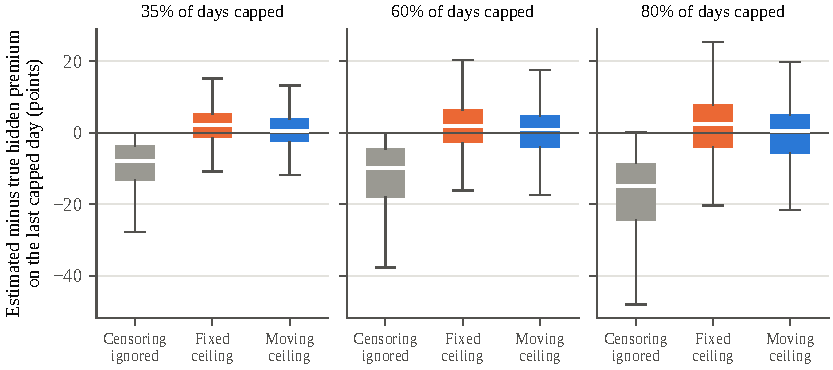
\includegraphics[width=0.8\textwidth]{figures/fig4_montecarlo.pdf}
\caption{Monte Carlo: error in the estimated hidden premium on the last capped day, by estimator and by the share of days capped. Boxes show the interquartile range and the median, whiskers 1.5 times the range. \mcReps{} replications per design; simulated data.}\label{fig:mc}
\end{figure*}

\subsection{Supply and float (P3)}
Each dated creation is a supply shock of known size. For every creation event $e$ in fund $i$, the change in the premium from five sessions before to ten sessions after is divided by the percentage change in units, which gives an elasticity $\eta_{i,e}=\Delta\pi_{i,e}/\Delta\ln(\text{units}_{i,e})$. Pooled within a fund, the elasticity implies the increase in units, and so the quota in dollars, that would have closed that fund's premium. The test that creations lower the premium is one-sided and is refuted by a zero or positive mean. Because room is shared within a fund house, outflows from sister schemes are examined as a source of variation in the capacity to create; the premium on each creation date is reported, and market makers are not identified. Across funds the relation between premium and net float is shown as a figure and tested with a rank correlation on the first session of each month after the change. With six funds a regression would add nothing to the picture.

\subsection{Limit-hit dynamics and feeders (S1, S2)}
For the sessions after the change,
\begin{equation}\label{eq:s1}
\begin{split}\Delta\pi_{i,t}&=a_i+b_1\,\mathit{TO}_{i,t}+b_2\,d_{i,t}+b_3\,r_{i,t-1}\\&\quad+b_4\,r_{i,t-5:t-1}+b_5\,A_t+\sum_{j=1}^{3}g_j\,H_{i,t-j}+\varepsilon_{i,t},\end{split}
\end{equation}
with turnover $\mathit{TO}$, delivered share $d$, the fund's own return over the previous one and five sessions, search interest $A$, and indicators $H$ for an upper-limit day $j$ sessions earlier. Resale-option models predict that premium and turnover rise together; extrapolation predicts a positive $b_3$ that survives the inclusion of turnover \citep{pearson2021chinese}; the attention account predicts positive $g_j$ with more and smaller trades. Errors allow for correlation across funds within a day \citep{driscoll1998consistent}. For feeders, the monthly change in ETF units held is set against the lagged premium; with a handful of feeders the evidence is descriptive.

\subsection{What the rule cost buyers}
A policy reader will ask what was paid above the price the old rule would have allowed. For each fund-day after the change,
\begin{equation}\label{eq:excess}
\begin{split}\text{excess rupees}_{i,t}&=\text{units traded}_{i,t}\\&\quad\times\max\big(0,\;\overline{P}_{i,t}-1.2\,\NAV_{i,t-2}\big),\end{split}
\end{equation}
where $\overline{P}_{i,t}$ is the day's average traded price. Summed by fund and week it measures the transfer from buyers to sellers that the old ceiling would have prevented, without any claim about who they were.

\subsection{Inference}
There are at most six treated funds from three fund houses and one rule date. Standard errors clustered by fund are unreliable at this number, as is the wild cluster bootstrap \citep{mackinnon2018wild}. The paper therefore leads with the holiday observation, the rank of the true date among placebo dates and break dates by fund, and uses panel estimates only in support. Tests are few and stated in advance, in the spirit of pre-analysis plans \citep{olken2015promises,harvey2017presidential}.

%=====================================================================
\section{Evidence Available Before the Panel}\label{sec:evidence}
This section reports what can be established now. Tables~\ref{tab:lastday}, \ref{tab:units} and~\ref{tab:cross} are computed from files of the exchange and of the Association of Mutual Funds in India for a few dates, saved by the project as test data for its collectors \citep{nse2026files,amfi2026nav}. Table~\ref{tab:path} mixes those files with press figures and says which is which. None of it tests a hypothesis.

\subsection{The last day of the fence}
The security master dated 4 September 2026 gives each fund's band for 7 September, the first session of the new regime. The band is 10\% either side of the 4 September close, with the lower limit rounded up and the upper rounded down to the paisa, so the close can be recovered exactly. The NAV file gives each fund's NAV for 2 September, and 1.2 times that NAV, rounded down, is the upper limit that applied on 4 September. Table~\ref{tab:lastday} compares the two.

\begin{table*}[!t]
\centering\footnotesize
\caption{The last session of the NAV-anchored band, 4 September 2026}\label{tab:lastday}
\begin{tabular}{lrrrcrr}
\toprule
 & NAV of & Upper limit, & Close, & Close at & NAV of & Quoted\\
Fund & 2 Sep (Rs) & $1.2\times$NAV (Rs) & 4 Sep (Rs) & the limit & 4 Sep (Rs) & premium (\%)\\
\midrule
\fund{MONQ50} & 118.2753 & 141.93 & 141.93 & yes & 118.7371 & 19.53\\
\fund{MON100} & 270.5591 & 324.67 & 324.67 & yes & 272.9167 & 18.96\\
\fund{MASPTOP50} & 66.5513 & 79.86 & 79.86 & yes & 66.7667 & 19.61\\
\fund{MAFANG} & 172.9741 & 207.56 & 207.56 & yes & 173.6007 & 19.56\\
\fund{MAHKTECH} & 18.4215 & 22.10 & 22.10 & yes & 18.5442 & 19.17\\
\fund{HNGSNGBEES} & 455.4774 & 546.57 & 471.09 & no & 459.4592 & 2.53\\
\addlinespace
\fund{NIFTYBEES} & 272.7284 & 327.27 & 273.27 & no & 272.5784 & 0.25\\
\bottomrule
\end{tabular}
\tabnote{Sources: \citet{amfi2026nav} for NAV; \citet{nse2026files} for the band applying on 7 September, from which the 4 September close is recovered as the only two-decimal price consistent with both limits. For \fund{MONQ50} the recovered close equals the close reported in the press. The quoted premium is the close over the NAV of the same date. \fund{NIFTYBEES} is a domestic ETF shown for comparison.}
\end{table*}

Five of the six funds closed at the upper limit to the paisa. NSE's close is the volume-weighted average of the last half hour, or the last trade if there was none, so a close exactly at the limit means that every trade in the closing half hour, or the last trade of the day, was at the limit price. Demand at the ceiling was unsatisfied in five funds on the day the ceiling was removed. The sixth, the Hang Seng fund, closed 2.5\% above NAV; its units have not changed since January 2025 either (Table~\ref{tab:units}), so a block on creation is not sufficient for a premium. Demand is also needed.

The table also shows the moving ceiling of Proposition~\ref{prop:fence} at work. All five funds were at the same limit of 1.2 times a lagged NAV, yet their quoted premiums range from 18.96\% to 19.61\%, because each fund's NAV had moved by a different amount over the two days.

\subsection{The path of one fund}
Table~\ref{tab:path} and Figure~\ref{fig:monq50} trace the Nasdaq Q50 ETF. On 7 September, with US markets shut, the fund's NAV changed by $-0.004\%$, the accrual of expenses, and its price rose 15.6\% \citep{vr2026rs96}: more than the initial 10\% band and the first widening allow, so the band widened twice on the first day. The close reached 235\% above NAV on 18 September, the ninth session. On 21 September the unit traded as high as Rs 471.99, 19.1\% above its base of Rs 396.30 and nearly four times that day's NAV, and closed at Rs 317.04, exactly 20\% below the base. About 4.3 million units changed hands, 29\% of all units outstanding \citep{indmoney2026penny,whalesbook2026}. No news, exchange action or fund-house statement has been reported as a trigger; the fall is treated here as endogenous. A second lower-limit day followed. By 7 October the premium was again above 110\%, and on 9 November the quoted premium was 100.8\%. The six funds together traded about Rs 10,440 crore on the two exchanges in 2026 up to early October, of which a press analysis places Rs 3,094 crore above NAV \citep{businessline2026}.

\begin{table*}[!t]
\centering\footnotesize
\caption{Motilal Oswal Nasdaq Q50 ETF: close, NAV and quoted premium, 2026}\label{tab:path}
\begin{tabular}{lrrrrl}
\toprule
Date & Session & Close (Rs) & NAV (Rs) & Premium (\%) & Source\\
\midrule
4 Sep & $0$ & 141.93 & 118.74 & 19.5 & Exchange and AMFI files\\
7 Sep & 1 & 164.07 & 118.73 & 38.2 & Close from reported rise; AMFI NAV\\
9 Sep & 3 & 213.01 & 116.42 & 83.0 & Press close; AMFI NAV\\
16 Sep & 7 & 275.28 & 116.69 & 135.9 & Press\\
17 Sep & 8 & 330.25 & 119.15 & 177.2 & Press\\
18 Sep & 9 & 396.30 & 118.14 & 235.5 & Press\\
21 Sep & 10 & 317.04 & 120.23 & 163.7 & Press\\
22 Sep & 11 & 253.64 & 120.17 & 111.1 & Press; value shown is iNAV\\
23 Sep & 12 & 202.92 & 120.59 & 68.3 & Press\\
30 Sep & 17 & 194.62 & 119.68 & 62.6 & Press\\
7 Oct & 21 & 258.57 & 123.09 & 110.1 & Press\\
14 Oct & 26 & 249.83 & 117.96 & 111.8 & Press\\
4 Nov & 40 & 219.38 & 117.76 & 86.3 & Press\\
9 Nov & 43 & 229.67 & 114.38 & 100.8 & Exchange and AMFI files\\
\bottomrule
\end{tabular}
\tabnote{Press sources: \citet{indmoney2026unwind,vr2026rs96,vr2026sep25,vr2026oct2,vr2026oct8,vr2026oct16,vr2026nov6}. Session counts NSE trading days from the change of anchor; 14 September was a market holiday. The close of 7 September is computed from the reported rise of 15.6\%. The premium is the close over the NAV shown. The press reported 81.4\% for 9 September using the NAV of 8 September.}
\end{table*}

\begin{figure*}[!t]
\centering
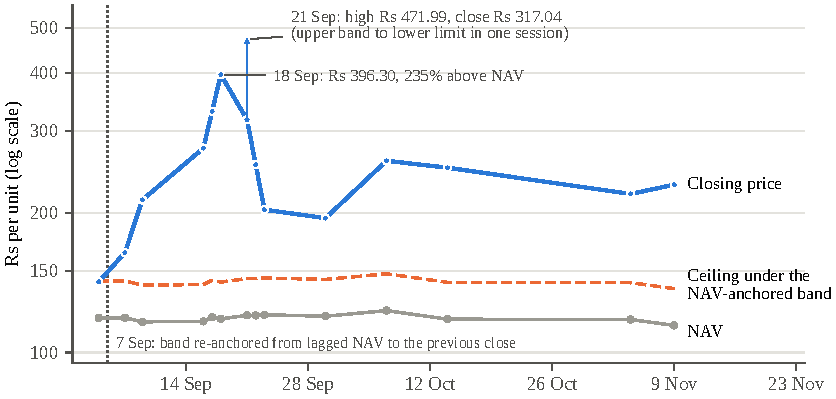
\includegraphics[width=0.95\textwidth]{figures/fig1_monq50.pdf}
\caption{Motilal Oswal Nasdaq Q50 ETF, 4 September to 9 November 2026: closing price, NAV and the ceiling that the NAV-anchored band would have set (1.2 times NAV). Points are the dates in Table~\ref{tab:path}; lines join them. The triangle marks the intraday high of 21 September.}\label{fig:monq50}
\end{figure*}

\subsection{Units outstanding}
Table~\ref{tab:units} reports units outstanding from NSE's security master on five dates. Between July 2024 and April 2026 the Nasdaq Q50 ETF's units rose from 3.28 million to 14.68 million, an increase of exactly 19 creation units, in a period that press accounts describe as closed to creation. Eight of the 19 came in the second half of 2024, when the fund's premium was reported between 17\% and 25\%; by May 2025 it had fallen to 1.8\% \citep{vr2025premium}. The Nasdaq 100 ETF added 26 creation units in the second half of 2024 and lost three afterwards. The Hang Seng fund added 179. The two Mirae Asset funds on US indices only shrank. From April to November 2026 no fund's units changed, although one creation unit of the Nasdaq Q50 ETF bought at NAV and sold at the 18 September close would have yielded about Rs 16.7 crore. The fund houses' room was exhausted when it would have been most valuable.

\begin{table*}[!t]
\centering\footnotesize
\caption{Units outstanding, millions}\label{tab:units}
\setlength{\tabcolsep}{5pt}
\begin{tabular}{lrrrrrr}
\toprule
 & & & & & & Change in\\
Fund & 1 Jul 2024 & 2 Jan 2025 & 1 Apr 2026 & 4 Sep 2026 & 9 Nov 2026 & creation units\\
\midrule
\fund{MONQ50} & 3.275 & 8.075 & 14.675 & 14.675 & 14.675 & $+19$\\
\fund{MON100} & 498.385 & 504.885 & 504.135 & 504.135 & 504.135 & $+26$, $-3$\\
\fund{MASPTOP50} & 172.474 & 168.624 & 168.624 & 168.624 & 168.624 & n.e.\\
\fund{MAFANG} & 253.304 & 248.904 & 247.304 & 247.304 & 247.304 & n.e.\\
\fund{MAHKTECH} & 192.912 & 192.912 & 193.712 & 193.712 & 193.712 & $+1$\\
\fund{HNGSNGBEES} & 19.112 & 23.587 & 23.587 & 23.587 & 23.587 & $+179$\\
\bottomrule
\end{tabular}
\tabnote{Source: \citet{nse2026files}, field \texttt{IssdCptl}; the value for 1 April 2026 is from the project's log of the same file series. Creation-unit sizes as in Table~\ref{tab:funds}; the two Mirae Asset funds on US indices lost 3.85 and 6.00 million units. Reconciliation with fund-house disclosures of assets is pending.}
\end{table*}

\subsection{The cross-section on 9 November 2026}
Table~\ref{tab:cross} is a snapshot of all six funds on the most recent date for which files are held. Three things stand out.

\begin{table*}[!t]
\centering\footnotesize
\caption{The six funds on 9 November 2026}\label{tab:cross}
\setlength{\tabcolsep}{3.9pt}
\begin{tabular}{lrrrrrrrr}
\toprule
 & & \multicolumn{2}{c}{Premium (\%) over} & Value & Value above & Turnover & Delivered & Rupees\\
\cmidrule(lr){3-4}
Fund & Close (Rs) & same-date & last known & at NAV & NAV & (\% of & share & per\\
 & & NAV & NAV & (Rs crore) & (Rs crore) & units) & (\%) & trade\\
\midrule
\fund{MONQ50} & 229.67 & 100.8 & 107.1 & 168 & 169 & 1.87 & 44.5 & 7,514\\
\fund{MASPTOP50} & 96.52 & 50.5 & 53.4 & 1,082 & 546 & 0.35 & 57.8 & 6,770\\
\fund{MAFANG} & 234.91 & 47.2 & 51.4 & 3,945 & 1,864 & 0.39 & 45.9 & 12,251\\
\fund{MAHKTECH} & 21.93 & 34.7 & 33.4 & 315 & 109 & 0.27 & 65.2 & 2,427\\
\fund{MON100} & 298.59 & 16.6 & 20.6 & 12,911 & 2,142 & 0.19 & 52.0 & 12,529\\
\fund{HNGSNGBEES} & 455.52 & 4.3 & 4.2 & 1,030 & 45 & 0.13 & 62.5 & 4,580\\
\addlinespace
Six funds & & & & 19,451 & 4,875 & & & \\
\addlinespace
\fund{NIFTYBEES} & 285.01 & $-0.3$ & $-0.2$ & 73,920 & $-208$ & 0.44 & 54.2 & 43,556\\
\bottomrule
\end{tabular}
\tabnote{Sources: \citet{nse2026files} for prices, traded quantity and value, trades, delivered share and units outstanding (NSE only); \citet{amfi2026nav} for NAV dated 9 November. The last known NAV is the NAV displayed by NSE at the close. Value at NAV is units times the NAV dated 9 November; market value above NAV is units times the close, less value at NAV. \fund{NIFTYBEES} is a domestic ETF shown for comparison.}
\end{table*}

First, the sums involved are not small. The six funds held assets worth Rs 19,451 crore at NAV and were priced Rs 4,875 crore above that, a quarter of their value. The largest amounts are in the large funds with moderate premiums, not in the fund with the headline premium: the Nasdaq 100 ETF and the FANG+ ETF account for Rs 4,006 crore of the total. This is what holders stand to lose if premiums close, whether through new room under the cap or through the return of a NAV anchor.

Second, among the four funds on US indices the smallest float carries the largest premium and the largest float the smallest (Figure~\ref{fig:cross}). The Nasdaq Q50 ETF, worth Rs 168 crore at NAV, turned over 1.9\% of its units in a day, ten times the rate of the Nasdaq 100 ETF, and had the lowest delivered share. Small float, high turnover and a large premium together are what models of speculative trading under short-sale constraints predict \citep{hong2006asset}. The figures are gross of feeder holdings and for one day; they motivate P3 and do not test it.

Third, the trades are small. The average trade in the six funds was between Rs 2,400 and Rs 12,500, against Rs 43,600 in the largest domestic ETF. Daily files do not identify investors, but trades of this size are not those of institutions.

\begin{figure*}[!t]
\centering
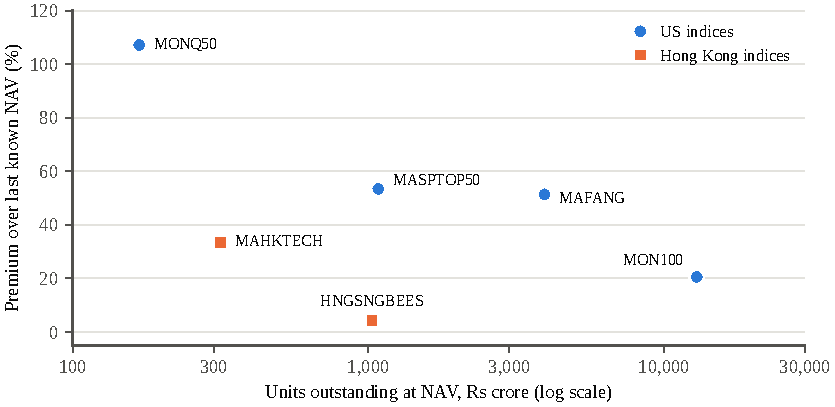
\includegraphics[width=0.92\textwidth]{figures/fig6_cross_section.pdf}
\caption{Premium and float on 9 November 2026. Premium over the last known NAV against units outstanding valued at NAV, gross of feeder holdings (Table~\ref{tab:cross}).}\label{fig:cross}
\end{figure*}

\subsection{Reading}
These figures are consistent with P1 and with the supply side of P3, and they contradict the common account that creation has been shut since 2022 or 2024. They do not test either. The premiums between the two file dates are press premiums with the timing defect of Section~\ref{sec:institutions}, units are observed on five dates, and no fair-value series has been computed. What the files do settle is the starting point for P2: on the day the fence came down, five funds were pressed against it.

%=====================================================================
\section{Registered Tests for April 2027}\label{sec:april}
Paragraph 4.4 of the circular makes the previous day's NAV the base from 1 April 2027, subject to exchanges and fund houses resolving operational difficulties. If any NAV anchor is applied, Proposition~\ref{prop:cliff} holds: a fund trading more than 20\% above the anchoring NAV must jump into the band on the first day. A holder who is certain of the switch should not hold through it. The switch is a target, however, and may be delayed, so a premium above the future ceiling is not by itself evidence of irrationality. The tests concern how the excess over that ceiling moves, and they are fixed here before any observation from 2027 exists. The text below will be filed on a public registry before 31 December 2026.

\paragraph{Definitions} The \emph{excess} of a fund on a day is
\begin{equation}\label{eq:xapril}
x_{i,t}=\ln\!\left(\frac{P_{i,t}}{1.2\times\NAV^{\mathrm{pub}}_{i,t}}\right),
\end{equation}
where $\NAV^{\mathrm{pub}}_{i,t}$ is the last NAV published before that close. An \emph{exposed fund} is one of the six with $x>0$ at the close of the last session of December 2026. The \emph{switch date} $T$ is the first session on which NSE's official band for a fund is centred on a NAV of any lag, read from the security master. An \emph{event} is a dated publication by SEBI, the Reserve Bank of India, NSE, BSE, the Association of Mutual Funds in India or the three fund houses about the band's base, the overseas limits or creation in these funds. Each event is logged with its time and classed, before prices are examined, as premium-reducing (anchor confirmed or advanced, limits raised, creation resumed) or premium-preserving (delay, exemption).

\paragraph{Branches} A: a NAV anchor is applied to these funds on or before 30 April 2027. B: a delay or exemption is announced before $T$. C: the limits are raised, or an exposed fund's units rise by at least one creation unit, before $T$.

\paragraph{Predictions} Each prediction names the branch in which it applies.\nopagebreak
\begin{enumerate}
\item \emph{Run, not cliff} (A). For every exposed fund $x\le 0$ at the close of $T-1$. The prediction is refuted for a fund if $x>0$ then, in which case the fall arrives as a jump on $T$.
\item \emph{Path} (A). Between 1 January and $T-1$ each exposed fund has at least one session whose low equals the official lower limit, and its median $x$ over the last 10 sessions before $T$ is below its median over sessions 11 to 40 before $T$.
\item \emph{News} (all branches). Across events and exposed funds, $x$ falls from the close before an event's first tradable session to the close two sessions later for premium-reducing events and rises for premium-preserving ones. An exact sign test is applied to the pooled changes.
\item \emph{Trading} (A, B). Units traded over units outstanding in the 20 sessions before $T$, or before the announcement in branch B, exceed the ratio in sessions 21 to 60 before.
\item \emph{Supply} (C). After units rise, $x$ falls, and by more where the percentage rise in units is larger.
\end{enumerate}
All five predictions will be reported whatever the result.

\paragraph{Known when written} Press premiums from 4 September to 4 November 2026; exchange and fund-industry files for 4 September and 9 November 2026; units outstanding on five dates; a check of NAV timing for one fund; no price after 9 November 2026; no output of the study's pipeline. This paragraph will be updated on the day of filing.

\paragraph{Why a run is the prediction} Before $T$ a falling price can lose at most 20\% a day, and on lower-limit days sellers may find no buyers, as on 21 and 22 September 2026. A fund at twice its ceiling needs at least four such sessions to get inside the band (Proposition~\ref{prop:cliff}). Holders who intend to leave must therefore leave early, and each has reason to leave before the others. The alternative is that the premium survives to $T-1$ because holders doubt the date, cannot coordinate \citep{abreu2003bubbles} or do not know the rule. The first prediction separates the two.

%=====================================================================
\section{Threats to Validity and Limitations}\label{sec:limits}
\emph{Few funds.} Six funds from three fund houses cannot support claims about ETFs in general. The contribution is a well-identified case, and inference is chosen accordingly.

\emph{A shared demand shock.} Chinese ETFs on US technology indices also traded at high premiums in September and November 2026 \citep{caixin2026nov}. A global rush into US technology shares could raise premiums in both countries. The China comparison is meant to separate that shock from the Indian rule; it is imperfect because Chinese quotas and subscription limits also changed during the year.

\emph{The latent premium is a model.} The split in~\eqref{eq:split} is relative to a law of motion estimated before the change. If that law would have changed in September 2026 for reasons unrelated to the rule, the change is counted as induced. The covariates, the China comparison and the two-sided form of the test limit the problem and do not remove it.

\emph{Fair value.} Three of the indices have no liquid future of their own, and the exchange rate each fund house uses is not yet documented. Errors of one or two percentage points do not matter at premiums above 50\% but do matter for the censored model near 20\%, which is why results are reported with unit and estimated betas and with the premium over the last known NAV.

\emph{Who buys.} Daily data show delivered share, trade count and trade size, not investor identity. Without account-level data the trading hypotheses distinguish mechanisms only indirectly, and the paper makes no statement about the rationality of any group.

\emph{Short selling.} Eligibility for securities lending is set by rule: an index ETF qualifies if it traded on at least 80\% of days over six months with an impact cost of 1\% or less \citep{bs2012slb}, and the Nasdaq 100 ETF was among the first admitted \citep{bs2013slb}. Three facts remain to be established for 2026: whether the six funds were on the eligible list, whether any units were in fact lent, and whether brokers allowed short sales within the day. Until they are, the paper says only that an overnight short position needed a borrow that we could not observe.

\emph{The rule may change.} SEBI may alter the April target or the limits. The branches in Section~\ref{sec:april} treat each as an event; they do not remove the uncertainty.

\emph{Sources.} Section~\ref{sec:evidence} uses press figures between its two file dates. The date on which the first band regime began has not been established and will be inferred from prices. How fund houses allocate freed room is not public.

\emph{Researcher knowledge.} P1 to P3, S1 and S2 were written after the September and October price path was public. They are predictions only for data not yet assembled. R1 is a prediction in the full sense.

%=====================================================================
\section{Conclusion}\label{sec:conclusion}
India's international ETFs offer an unusual setting: an asset with a published value, a regulatory barrier to arbitrage that can be dated from exchange records, and a price limit whose anchor moved once and is due to move again. The argument of this paper is that the anchor is not a technical detail. Anchored to value, a limit bounds mispricing; anchored to price, it bounds only the speed at which mispricing can grow; and a return from the second to the first forces a jump. Files for the last day of the old rule show five of six funds pressed against the ceiling, and files for 9 November show holders owning units priced Rs 4,875 crore above what the funds hold.

How much of that premium was waiting behind the fence and how much the new rule created is the question the design is built to answer, with an estimator that recovers a known hidden premium in simulation and a test whose size will be calibrated by bootstrap. The next version of the paper will report the estimates. The version after April 2027 will report the outcome of the registered tests, whichever way they fall.

For regulators the case carries a general point. A rule written for assets whose price can outrun a stale value was applied to assets whose price is not tied to value at all, and the property that had kept them near value was a side effect of the rule that was replaced. Where creation can be blocked, a limit on price changes is not a limit on mispricing, and some instrument anchored to value, whether a band, a halt or a call auction, has to do that job.

%=====================================================================
\appendix
\section{Protocol Timeline}\label{app:protocol}
Table~\ref{tab:protocol} lists, for each element of the design, the date it was fixed and what had been seen at that date.

\begin{table*}[!t]
\centering\footnotesize
\caption{Elements of the design and outcomes already seen}\label{tab:protocol}
\begin{tabularx}{\textwidth}{L{3.9cm}L{2.6cm}Y}
\toprule
Element & Date fixed & Outcomes seen at that date\\
\midrule
Fair-value measure \eqref{eq:fv}, \eqref{eq:pi} & 10 Nov 2026 & NAV timing check for one fund; no fair-value series computed\\
P1 to P3, S1, S2; the window of sessions 16 to 40 in \eqref{eq:iota} & 11 Nov 2026 & Press premiums, 4 Sep to 4 Nov 2026; units outstanding on five dates; no output of the study's pipeline\\
Estimator of Section~\ref{sec:design}, its Monte Carlo check and the bootstrap calibration & 12 Nov 2026 & As above, plus exchange and fund-industry files for 4 Sep and 9 Nov 2026 (Tables~\ref{tab:lastday} and~\ref{tab:cross}); simulated data only\\
R1 and the tests of Section~\ref{sec:april} & 11 Nov 2026 (text); registration pending & As above; no price after 9 Nov 2026\\
\bottomrule
\end{tabularx}
\end{table*}

\section{Monte Carlo Design}\label{app:mc}
\emph{Data-generating process.} The latent log premium follows $\pi^{*}_{t}=\mu(1-\rho)+\rho\pi^{*}_{t-1}+\sigma\varepsilon_t$ with $\rho=0.985$, $\sigma=0.02$ and $\mu\in\{0.10,0.20,0.30\}$, started from its stationary distribution. Daily log changes in value are $n_t\sim N(0,0.012^2)$ and the ceiling is $c_t=\ln 1.2-(n_t+n_{t-1})$. For $t\le 400$ the observed premium is $\min(\pi^{*}_t,c_t)$. A replication is kept if the last pre-change day is capped and between 10\% and 95\% of pre-change days are capped. For $t>400$ the observed premium is $\pi^{*}_t+\delta$ with $\delta\in\{0,0.3,0.6\}$.

\emph{Estimators.} (i) Ordinary least squares of the observed premium on its lag. (ii) Maximum likelihood for~\eqref{eq:latent}--\eqref{eq:obs} applied to the premium over the band's base, $\pi_t+(n_t+n_{t-1})$, with the fixed ceiling $\ln 1.2$. (iii) Maximum likelihood for~\eqref{eq:latent}--\eqref{eq:obs} with the moving ceiling $c_t$. For (ii) and (iii) the likelihood is computed by the recursion~\eqref{eq:filter} on a grid of 193 points from 0.02 to 1.30 and maximised by the Nelder--Mead method from the least-squares estimates.

\emph{Outcomes.} The hidden premium on day 400 is the mean of the filtered density, compared in levels with the true latent premium. The forecast is 1,500 paths simulated from the filtered density; the 5th and 95th percentiles of the average log premium over sessions 16 to 40 form the band. The plug-in band holds the parameters at their estimates. The band with parameter uncertainty draws one parameter vector per path from a normal distribution centred on the estimates, with the inverse numerical Hessian of the log-likelihood as covariance (for the first estimator, the least-squares covariance). The induced share is~\eqref{eq:iota}. The true induced share is computed from the simulated latent path. The code, \texttt{mc\_censored.py}, is in the \texttt{analysis} folder beside the source of this paper; seeds are fixed, and a replication takes about four seconds.

\section{Variable Definitions}\label{app:variables}
\begin{table*}[!t]
\centering\footnotesize
\caption{Variables in the fund-day panel}\label{tab:variables}
\begin{tabularx}{\textwidth}{L{3.2cm}YL{3.4cm}}
\toprule
Variable & Definition & Source\\
\midrule
Close, last, high, low, average price & NSE daily prices; the close is the average of the last half hour & NSE bhavcopy\\
Same-date NAV & NAV dated $t$ & AMFI\\
Last known NAV & Last NAV whose underlying market had closed before 15:30 on $t$, with its date & AMFI, calendars\\
Fair value $\FV$ & Last known NAV moved to 15:30 by the index future and the rupee rate, eq.~\eqref{eq:fv}, with $\beta=1$ and with estimated $\beta$ & Terminal export\\
Premium $\pi$ & $\ln(\text{close}/\FV)$; main dependent variable & Derived\\
Quoted premium & Close over same-date NAV, less one; for comparison with the press only & Derived\\
Band low, band high & Official band for session $t$ & NSE security master of the previous session\\
Ceiling $c$ & $\ln(\text{band high}/\FV)$, eq.~\eqref{eq:cap} & Derived\\
Limit indicators & High at the initial upper limit; at the maximum limit; last trade at the limit; and the same for the lower limit & Derived\\
Regime & Base that reproduces the band's midpoint: NAV of $t-2$, previous close, NAV of $t-1$ & Derived\\
Units & Units outstanding: daily from July 2024; monthly assets over NAV before & NSE security master; fund houses\\
Creation event & Signed change in units over the creation-unit size & Derived\\
Rationed & One when $\pi>0.02$ and no creation in the previous 20 sessions & Derived\\
Feeder units & ETF units held by feeder funds, monthly, carried forward & Monthly portfolios\\
Net float & (Units less feeder units) times last known NAV & Derived\\
Turnover & Units traded on NSE and BSE over units outstanding & NSE, BSE\\
Delivered share, trades, trade size & Share of traded quantity delivered; number of trades; value per trade & NSE bhavcopy\\
Own returns & Log price return over the previous one and five sessions & Derived\\
Attention & Google Trends daily index for fixed terms, chained across windows & Google Trends\\
Excess $x$ & $\ln(\text{close}/(1.2\times\text{last published NAV}))$, eq.~\eqref{eq:xapril} & Derived\\
Excess rupees & Units traded times $\max(0,\text{average price}-1.2\times\NAV_{t-2})$, eq.~\eqref{eq:excess} & Derived\\
\bottomrule
\end{tabularx}
\end{table*}

\section{Chronology}\label{app:chronology}
\begin{table*}[!t]
\centering\footnotesize
\caption{Dated events}\label{tab:chronology}
\begin{tabularx}{\textwidth}{L{2.6cm}YL{3.3cm}}
\toprule
Date & Event & Source\\
\midrule
Apr 2008 & Industry limit on overseas investment by mutual funds set at US\$7 billion & \citet{lawasia2026}\\
5 Nov 2020 & Limit per fund house raised to US\$600 million & \citet{bs2020limit}\\
3 Jun 2021 & Limit per fund house raised to US\$1 billion; US\$300 million per house within US\$1 billion for foreign-listed ETFs & \citet{bs2021limit}\\
18 Jan 2022 & Motilal Oswal suspends issuance of units in its two Nasdaq ETFs & \citet{bs2022motilal}\\
1 Feb 2022 & Fresh overseas subscriptions stop across the industry & \citet{pti2022resume}\\
Jun 2022 & Funds may resume up to each house's room as of 1 February 2022 & \citet{pti2022resume}\\
8 Feb 2023 & Reserve Bank of India: no proposal to raise the limit & \citet{bs2023rbi}\\
5 Jan 2024 & Mirae Asset stops direct creation in its three overseas ETFs & \citet{mirae2024addendum}\\
1 Apr 2024 & Pool for foreign-listed ETFs full & \citet{zerodha2024etf}\\
5 Jan 2025 & Motilal Oswal pauses existing instalment plans in its Nasdaq 100 feeder & \citet{et2025motilal}\\
Oct 2025 & Silver ETFs trade about 10\% above indicative value in a shortage of metal; fund houses suspend feeder subscriptions & \citet{bs2025silver}\\
Late Jan 2026 & Gold and silver outrun the NAV-anchored band; interim base for bullion ETFs & \citet{sebi2026cp}\\
13 Feb 2026 & SEBI consultation paper on base price and bands & \citet{sebi2026cp}\\
15 Jun 2026 & SEBI circular: base is the previous close; NAV base targeted for 1 April 2027 & \citet{sebi2026circular}\\
28 Aug 2026 & Start moved from 1 to 7 September & \citet{sebi2026ext}\\
1 Sep 2026 & NSE implementing circular & \citet{nse2026circular}\\
4 Sep 2026 & Last session of the NAV-anchored band; five of six funds close at the upper limit & Table~\ref{tab:lastday}\\
7 Sep 2026 & Previous-close anchor in force; US markets closed & \citet{nse2026files}\\
18 Sep 2026 & Nasdaq Q50 ETF closes 235\% above NAV & \citet{indmoney2026unwind}\\
21--22 Sep 2026 & Nasdaq Q50 ETF: two lower-limit closes & \citet{indmoney2026unwind}\\
25 Sep 2026 & NSE and BSE press releases cautioning investors & \citet{nse2026press,bse2026press}\\
7 Oct 2026 & NSE repeats its caution & \citet{reuters2026nse}\\
9 Nov 2026 & Six funds priced Rs 4,875 crore above NAV & Table~\ref{tab:cross}\\
1 Apr 2027 & Target date for a base of the previous day's NAV & \citet{sebi2026circular}, para.\ 4.4\\
\bottomrule
\end{tabularx}
\end{table*}
